\documentclass[runningheads]{llncs}
\usepackage{graphicx}
\usepackage{float}
\begin{document}
\begin{titlepage}
\centering
{\scshape\LARGE University of Potsdam \par}
\vspace{1cm}
{\scshape\Large Final Thesis for a Bachelor's Degree in Computational Science\par}
\vspace{1.5cm}
{\huge\bfseries Map Abstraction for Multi-Agent Pathfinding problems with Answer Set Programming\par}
\vspace{2cm}
{\Large\itshape Adrian Salewsky\par}
\vfill
supervised by\par 
\vspace{\baselineskip}
Prof Torsten Schaub \\
\vspace{\baselineskip}
Arvid Becker
\vfill
{01.04.2022 \par}

\begin{abstract}
Multi-Agent Pathfinding stellt ein wichtiges Problem in der Informatik dar. Folglich wird versucht, die Geschwindigkeit von Lösungs- \\
algorithmen ständig zu verbessern.
In dieser Arbeit stelle ich meine Methode zur Kartenabstraktion für solche Probleme dar und zeige auf, wie diese genutzt werden können, um entsprechende Probleme
schneller zu lösen. Es wurde das deklarative Programmierparadigma Answer Set Programming genutzt, um die Abstraktion zu bilden. Weiterhin wurde Python verwendet, um verschiedene Hilfsprogramme zu erstellen.
Als Vergleichswert für die Lösungszeit wurde das Framework ``asprilo'' genutzt, das ebenfalls die Sprache Answer Set Programming nutzt. Die Arbeit wurde in englischer Sprache verfasst. 		
\end{abstract}
\end{titlepage}


\section{Introduction}
Multi-Agent Pathfinding (MAPF) is an important problem in computer science. Therefore, it is important to look for ways to improve the solving time of such problems. One way to do that is to abstract the instance that has to be solved to reduce the size of
possible plans. This paper will show how I built such abstractions in the declarative programming paradigm ``Answer Set Programming'' (ASP). In the next two sections, I will explain MAPF problems and how ASP works. After that, I will introduce the ``asprilo'' framework used as a base for the enoding. It also serves as a comparison for the solving time. Then, I will explain how my abstraction methods work, and how the results of these abstractions look. I will also briefly skim over some additional programs that provided support for the solving. Following that, I will show the benchmarking results of the methods. I will end the paper with a conclusion of my work. \\
All the used programs and instances can be found in my GitHub repository \cite{my-git}. This paper was written as the final thesis for a Bachelor's degree in the course Computational Science at the University of Potsdam. This project was done in cooperation with Tarek Ramadan who worked on using the abstractions to solve a problem as a project for his final thesis for a Bachelor's degree in the same course and university. His work can be found on his GitHub repository \cite{tarek-git}.

\section{Multi-Agent Pathfinding}
In Multi-Agent Pathfinding problems, you have a set of nodes, agents (e.g. robots), start and goal positions, and possible moves. The set of nodes declares the possible positions where robots can be and move to. The robots can move from one node to accessible neighboring nodes in discrete time steps. In this paper, only orthogonal moves are considered. The goal is to let each robot find a way from its start to its goal position. It is possible to not have predetermined goal positions for each specific robot and instead let the solver assign the goal positions to the robots that can have the best way to that position. I only dealt with having a predetermined goal position for each robot in this project. The result of the solving process is a plan with a set of moves for each robot. When executing the plan there must not be any collisions. Possible collisions are edge collisions (robots moving through each other) and vertex collisions (robots moving to the same node) (see figure \ref{fig:mapf}). The last time step of the plan is called horizon or makespan \cite{mapf}. 

\begin{figure}[h]
\centering{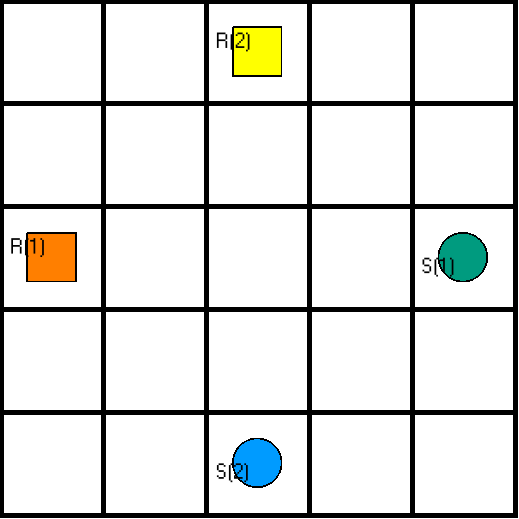
\includegraphics[scale=.4]{Images/MAPF-Problem}}
\caption{Robot 1 (the square on the left) has to reach shelf 1 (the circle on the right). Robot 2 has to reach shelf 2 The shortest path is to go right/down 4 steps. In the middle, a conflict would occur which could be avoided by letting one robot wait for one time step.}
\label{fig:mapf}
\end{figure}

\section{Answer Set Programming}
Answer Set Programming is a declarative programming paradigm that is especially useful when using it for NP-hard search problems. For a complete introduction refer to \cite{asp}. In this section, I will only briefly explain the main parts relevant to my encoding. \\
An ASP program contains a set of rules and atoms. The result is a stable model that is built upon these rules and atoms. An atom has the form: 
\begin{verbatim}
a.
\end{verbatim}
This means that the $a$ is treated as a fact and always has to be true. Rules have the form:
\begin{verbatim}
b :- a.
\end{verbatim}
which means that if $a$ is true then $b$ also has to be true. There are also negations:
\begin{verbatim}
b :- not a.
\end{verbatim}
This means that $b$ can only be inferred if $a$ is never true in the model. There are also choice rules:
\begin{verbatim}
x {b,c,d} y :- a.
\end{verbatim}
The atom $a$ is used to infer the choice rule. The solver can then decide which of the atoms $b$, $c$, and $d$ he wants to infer. He can also decide to not choose any atoms at all. You can set bounds for the number of atoms chosen. In this case, it means that the solver has to at least choose $x$ atoms, and cannot choose more than $y$ atoms. You can also influence the chosen atoms by using constraint rules of the form:
\begin{verbatim}
:- a, b.
\end{verbatim}
This means that $a$, and $b$ cannot be true at the same time. Combining this constraint rule with the choice rule above means that the solver will not choose to infer $b$. Atoms can also have attributes:
\begin{verbatim}
a(1). a(2).
\end{verbatim}
This means that there is an atom $a$ with the attribute $1$, and an atom $a$ with the attribute $2$. In rules you can exchange the attributes with variables:
\begin{verbatim}
b(X) : a(X).
\end{verbatim}
This means that the solver looks for every atom $a$ with exactly one attribute and infers the atom $b$ with the same attribute. Before the solver looks for stable models, the program is $grounded$. During this process, the variables in the program are exchanged with the actual values. \\
The last form of rule to talk about is called aggregates. I will explain two aggregates that have also been used in the abstraction encoding. The first one is $min$:
\begin{verbatim}
a(MIN) :- MIN == #min{X: b(X)}.
\end{verbatim}
The solver looks for the attribute of the atom $b$ with the lowest value and assigns  $MIN$ this lowest value. It then infers the atom $a$ with the attribute $MIN$. The other aggregate, I used in my encoding is $minimize$:
\begin{verbatim}
#minimize {X : a(X)}.
\end{verbatim}
This means that the solver looks at every atom $a$ with one attribute and builds the sum of these attributes. It then looks for the model with the lowest sum. \\
There are also other aggregates that I have not explained but since I do not use them in my encoding, I will not explain them. An ASP program has the file ending $.lp$.\\
To ground and solve the programs in this paper, clingo-5.4.0 was used \cite{clingo}. 



\section{Asprilo}
The asprilo framework is an ASP-based framework that is used to create plans for robots in a warehouse situation. It was created by Potassco. There are multiple domains in the framework. The domain that is important for this paper is the M-domain where only simple robot movement is important which turns the problem into a MAPF-problem. In the M-domain there are robots and shelves. Both have predetermined starting positions. The robots can move orthogonally. The goal is that each shelf is occupied by a robot when the time horizon is reached. Other domains also consider having the robots move the shelves around or having a robot battery but this is not important when dealing with simple MAPF-problems. The asprilo encoding serves as a base for my encoding which is why I will explain the different parts of the encoding that are relevant for my programs in the following subsections. The encoding and a complete guide can be found on the website by Potassco \cite{asprilo}.
\subsection{Instances}
 Since the M-domain only needs nodes, robots and shelves, only these are initiated:
\begin{verbatim}
init(object(node,N),value(at,(X,Y))).
init(object(robot,R),value(at,(X,Y))).
init(object(shelf,S),value(at,(X,Y))).
\end{verbatim}
The first line is used to initiate a node with the ID $N$ at the position $X, Y$. $X$ and $Y$ are the coordinates for a 2-dimensional grid. The second and third lines are used to initiate a robot with the ID $R$ and a shelf with the ID $S$ respectively. The IDs are usually integers so the first robot, shelf, or node would usually get the ID 1, the second gets the ID 2, and so on. \\
That is all that needs to be initiated for the M-domain. If a node between two other nodes is not initiated, it is treated as a wall.
\subsection{Input}
The program $input.lp$ is used to turn the $init$-atoms into others that are easier to work with:
\begin{verbatim}
robot(R) 			:- init(object(robot,R),_).
isRobot(robot(R)) 		:- robot(R).
position((X,Y))   		:- init(object(node,_),value(at,(X,Y))).
position(R,(X,Y),0) 		:- init(object(robot,R),value(at,(X,Y))).
position(shelf(S),(X,Y),0)	:- init(object(shelf,S),value(at,(X,Y))).
\end{verbatim}
The first line creates the $robot$-atom which simply states that the robot with ID $R$ exists. This is then used to create the atom $isRobot$ which can be used to check if an object is a robot. These two lines also exist for shelves. \\
The next three lines create the $position$-atoms. The first one takes just the information about the coordinates from the node initiation. The second one says that robot $R$ is on the position it is initiated on, i.e. his starting position, at time step 0 which is the first time step. The third one states that the shelf with ID $S$ is on its starting position, which then serves as a goal position, at time step 0. The shelves are not moved in the M-domain which is why the shelf position could have also been initiated without the time step but this way it is easier to change it to a higher domain. It is also important to note that instead of having just the ID as the first argument, it has $shelf(S)$. This makes it easier to distinguish between shelves and robots when using $position$.
\subsection{Action}
The program $action.lp$ is the one where moves are created. First off, the time array is created:
\begin{verbatim}
time(1..horizon).
\end{verbatim}
This line creates $time$-atoms with the arguments being rising integers starting from one until the constant $horizon$ is reached. This constant has to be given externally to the program.  \\
Then the possible directions are created:
\begin{verbatim}
direction((X,Y)) :- X=-1..1, Y=-1..1, |X+Y|=1.
nextto((X,Y),(DX,DY),(X',Y')) :- 
                               direction((DX,DY)), position((X,Y)), position((X',Y')),
                               (X,Y)=(X'-DX,Y'-DY), (X',Y')=(X+DX,Y+DY).
\end{verbatim}
The first rule initiates the four orthogonal movements as possible directions. The second rule states that a node is next to another one if it can be reached by going in one of the possible directions. \\
The next rule creates the actual $move$-atoms:
\begin{verbatim}
{ move(R,D,T) : direction(D) } 1 :- isRobot(robot(R)), time(T).
\end{verbatim}
This rule states that for each robot at each time step up to one move is created into one possible direction. It is also possible to not create a move at certain time step. Not moving is an action equivalent to waiting. These moves have to change the positions of robots accordingly:
\begin{verbatim}
position(R,C,T) :- move(R,D,T), position(R,C',T-1),     nextto(C',D,C).
                :- move(R,D,T), position(R,C ,T-1), not nextto(C ,D,_).
position(R,C,T) :- position(R,C,T-1), not move(R,_,T), isRobot(robot(R)), 
                             time(T).
\end{verbatim}
The first rule changes the position of the robot according to the move taken. The second rule states that a robot cannot move to a position that does not exist. The third rule states that if a robot has not moved at a certain time step, its position does not change at that step. \\
There are more rules not shown here, that prohibit vertex and edge conflicts. These rules are not important for my encoding which is why I will not explain them further. 
\subsection{Goal}
The goal condition of the normal M-domain states that at the last possible time step, i.e. horizon, each shelf must be occupied by a robot. For this project the goal condition was slightly altered so that a robot moves to the shelf with the same ID:
\begin{verbatim}
goal(R,C) :- isRobot(robot(R)), position(shelf(S),C,0), R=S.
:- isRobot(robot(R)), position(R,C,horizon), goal(R,C'), C!=C'.
\end{verbatim}
The first rule creates the $goal$-atom. It says that the goal of robot $R$ is the cell $C$ (cell is synonymous with node). The goal cell is the cell on which the shelf with the same ID as the robot is initiated. This means that the solver cannot decide which robot should go to which shelf but it is predetermined. The second rule states that a robot cannot be on a cell that is not its goal at the last time step.
\subsection{Output and Encoding}
The file $output.lp$ determines how the output of the program looks. I will not show the encoding since the output of my encoding is a different one. It is enough to know that the output of the asprilo encoding is a plan, i.e. atoms that state how each robot moves at each time step. \\
The last file $encoding.lp$ includes the other files important for solving (it does not include the input instance). This means it contains the complete solving program. My encoding follows the same file structure which I will show in the next section.
\subsection{Visualizer}
The visualizer is an extra component provided by asprilo. It can be used to visualize instances and the movement of robots. All images in this paper showing instances and robots have been created with this visualizer.

\section{Abstraction Methods}
I have developed four abstraction methods. All of them use some of the asprilo encoding as a base. The files $input.lp$ and $goal.lp$ are the same as in the modified asprilo encoding. \\
The output atoms are $new\_init$ and $imp\_position$. The $new\_init$ atoms describe the resulting abstracted instance. The form of $new\_init$ resembles that of the $init$ atoms in the input instance. There are $new\_init$ atoms for robots, shelves, and nodes. The ones
for robots and shelves are the same as in the input instance (with of course a ``new'' being added) since the start and goal conditions are not changed during the abstraction. The atoms for the nodes contain only the nodes that still exist after the abstraction. The $imp\_position(R, C)$ atom states that robot $R$ is on cell $C$ at some point while building the abstraction. This can be used as extra information when solving the instance with the use of this abstraction, e.g. a solver could look at this information to know a possible path for each robot. The output is the same for every method except for the ``Reachable Nodes'' method. In that method, the output is slightly different which I will explain in the respective subsection. \\
The first part of the abstraction building is always solving the instance without caring for conflicts. Therefore the encoding entails parts of the $action.lp$ asprilo encoding. The difference is that the constraint rules which prohibit conflicts are ignored.
Furthermore there are two extra lines:
\begin{verbatim}
:- move(R,_,T1), not move(R,_,T2), time(T2), isRobot(robot(R)), T2<T1.
#minimize {1,(R,T): move(R,_,T)}.
\end{verbatim}
The first line states that a robot must always move until it has finished moving completely. This ensures that a robot does not wait instead of going to its goal. \\
The second line is used to minimize the number of moves each robot does. This is used to ensure that the solver looks for the shortest paths of the robots. \\
In the following subsections, I will explain the idea behind each abstraction method and show the encoding that is only used in that method respectively. 
\subsection{Shortest Path}
The first method is to look for the shortest path for each robot to its respective goal. Each position the robot visits is then used to create the $imp\_position$ atoms. An example instance can be seen in figure \ref{fig:inst-bef-a}. The corresponding abstraction can be seen in figure \ref{fig:inst-aft-a}.
\begin{verbatim}
imp_position(R,C) :- position(R,C,_), isRobot(robot(R)).
\end{verbatim}
In this method, it is also possible to add the time step at which the robot visits the position as an argument to the $imp\_position$ atom. However, this would mean that a solver that uses the abstraction to solve the instance would need to specifically
be designed for the ``Shortest Path'' method. Always using the same structure for each method means that one solver can be created to work for all methods. It is also not possible to check how many arguments the atom has because the 
``Reachable Nodes'' method needs the third argument for something different, which I will explain in the respective subsection. If it is not of interest to have a solver that solves by using the different abstractions the same way, the line shown above can 
easily be modified to contain the information about the time step. The output would then have to be modified as well. \\
Of the methods explained in this paper, this is the one that results in the smallest abstraction. It could also be viewed as a special case of the other methods because the other methods can find the same solution if the parameters are selected accordingly. If there is a shortest path in an instance, this method will find it so it can be used for all solvable
MAPF problems. 

\begin{figure}[h]
\begin{minipage}{.4\linewidth} 
\centering{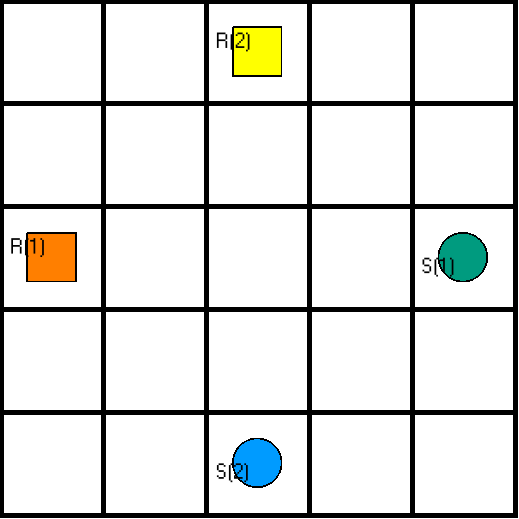
\includegraphics[scale=.4]{Images/MAPF-Problem}}
\caption{Input instance before abstraction}
\label{fig:inst-bef-a}
\end{minipage}
\hspace{.1\linewidth}
\begin{minipage}{.4\linewidth} 
\centering{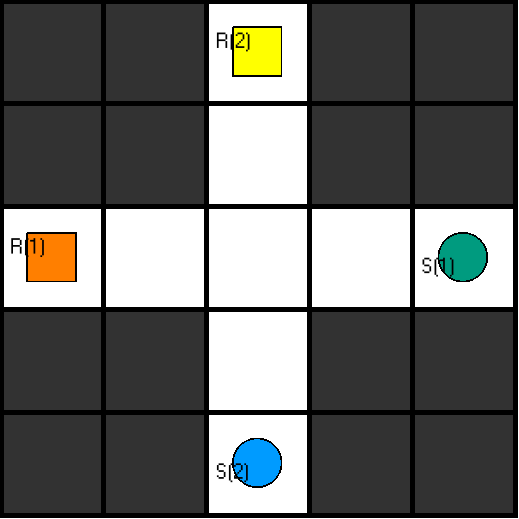
\includegraphics[scale=.4]{Images/SP-Example}}
\caption{Input instance after abstraction. Only the nodes that lie on the shortest path are considered}
\label{fig:inst-aft-a}
\end{minipage}
\end{figure} 


\subsection{Node Combining}
The idea for the node combining was taken from two other abstraction-related papers \cite{nc1} \cite{nc2}. The approach had to be slightly altered because my focus is to only build an abstraction and not solve the instance completely. The idea is to combine several nodes into one node (see figure \ref{fig:post-com} for illustration). Afterwards, the solver looks for the shortest path in the combined instance. The solver then outputs all the nodes that have been visited in the combined form (see figure \ref{fig:onc-result}). The respective encoding looks like this:
\begin{verbatim}
comb_position((X,Y),(X',Y'))   :- position((X,Y)),
          X' = (X+(size_x-1))/size_x, Y' = (Y+(size_y-1))/size_y.
comb_position(C)               :- comb_position(_,C).
comb_position(R,C',0)          :- position(R,C,0), comb_position(C,C').
comb_position(shelf(S),C',0)   :- position(shelf(S),C,0), comb_position(C,C').
\end{verbatim}
The first rule calculates the coordinates that a node has after combining. The constants $size\_x$ and $size\_y$ represent the predetermined amount of nodes that are combined in x- and y-direction respectively. The second rule is used so that it is not necessary to always care about the initial nodes. Rule 3 and 4 change the positions of robots and shelves to their new coordinates. The rest of the encoding is only changed so that the atoms $comb\_position$ instead of $position$ are used. The output atom $imp\_position$ is then easily inferred by looking at the positions visited by robots:
\begin{verbatim}
imp_position(R,C) :- isRobot(robot(R)), comb_position(R,C',_), comb_position(C,C').
\end{verbatim}
It takes the positions visited by robots, looks at the nodes that were combined into that position, and then infers the respective atoms. \\
Simply using this approach has the problem that walls are completely ignored while building the combined instance. This means that the encoding introduced so far can only be used for open instances, i.e. instances that do not have any inner walls. This is why I call this approach ``Open Node Combining''. The advantage of this method is that the combining size can be freely chosen, as long as positive integers are used. \\
To also use the node combining approach in instances with walls, I created the approach ``Complete Node Combining''. This approach mostly works the same but it can only be used when combining 2x2 squares together. The difference is that a $wall$-atom is introduced so that walls are considered after the combining:
\begin{verbatim}
wall((X1',Y1'),(X2',Y2')) :- comb_position((X1',Y1')), x_arr(X1), y_arr(Y1),
    not position((X1,Y1)), not position((X1+1,Y1)),
    X1' = (X1+(size_x-1))/size_x, Y1' = (Y1+(size_y-1))/size_y,
    X1'-1 = X1/size_x, Y1'-1 = Y1/size_y,
    comb_position((X2',Y2')), X1'=X2', Y1'-1=Y2'.
\end{verbatim}
This is one of four rules inferring a $wall$-atom. The idea is that in a 2x2 square there are four possible walls: two nodes missing to the top, bottom, left, or right. Each rule inferring a $wall$-atom is used for one of the possible walls. The rule takes a combined node and checks if there are exactly two uncombined nodes missing that would be in that combined node if they existed. The $nextto$-atom is then extended to also check if a wall is between two combined nodes before inferring the respective atom:
\begin{verbatim}
nextto((X,Y),(DX,DY),(X',Y')) :- dir((DX,DY)),
   comb_position((X,Y)), comb_position((X',Y')),
   (X,Y)=(X'-DX,Y'-DY), (X',Y')=(X+DX,Y+DY),
   not wall((X,Y),(X',Y')), not wall((X',Y'),(X,Y)).
\end{verbatim}
As mentioned before, this way of introducing walls leads to only being able to combine 2x2 squares. I did not find a way to combine bigger sizes because looking at walls in these cases gets much more complicated. \\

\begin{figure}[h]
\begin{minipage}{.4\linewidth} 
\centering{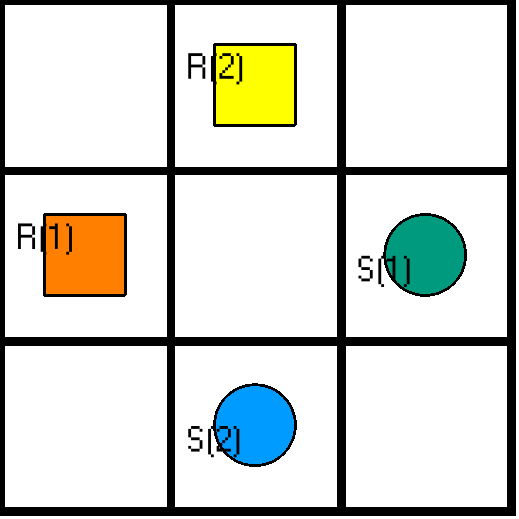
\includegraphics[scale=.4]{Images/Post-Combining-Example}}
\caption{The input instance can be seen in figure \ref{fig:inst-bef-a}. This image shows how the combined instance would look like if the combining size is set to 2x2.} 
\label{fig:post-com}
\end{minipage}
\hspace{.1\linewidth}
\begin{minipage}{.4\linewidth} 
\centering{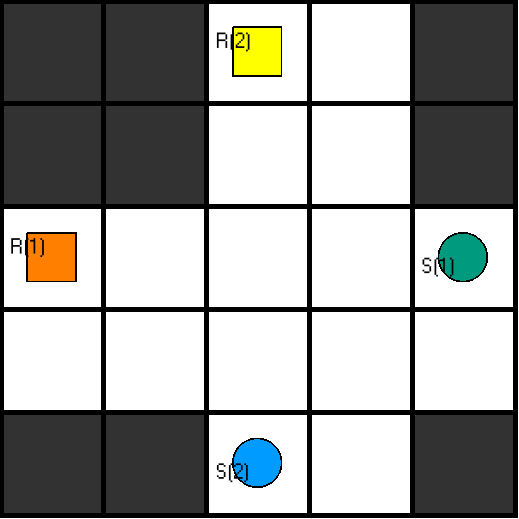
\includegraphics[scale=.4]{Images/ONC-2-2-Example}}
\caption{This image shows the resulting instance. Nodes that were not visited in combined form get deleted.}
\label{fig:onc-result}
\end{minipage}
\end{figure} 


\subsection{Reachable Nodes}
The last abstraction method was also inspired by a research paper \cite{rn}. Again, a slight alteration was done because the goal is to only find an abstraction and not a complete solution. The idea is to find the shortest path for each robot. Then, the solver looks at how many steps each node close to the path of the robots is deviating from that path. The path itself is deviating by zero steps. Each node next to the path is deviating by one step, the nodes right next to them by 2  steps, and so on (see figure \ref{fig:rn}). The maximum amount of steps looked at is the number of steps the robot needed in total to reach its goal. 
\begin{verbatim}
makespan(R,N) :- move(R,_,N).
imp_pos(R,C,0) 	:- isRobot(robot(R)), position(R,C,_).
imp_pos(R,C,N) 	:- isRobot(robot(R)), imp_pos(R,C',N-1), makespan(R,N), nextto(C',_,C).
imp_position(R,C,MIN) 		:- imp_pos(R,C,MIN), MIN == #min{X: imp_pos(R,C,X)}.
\end{verbatim}
The first line looks at how many steps each robot takes. It is important to note that makespan refers to an individual robot whereas horizon refers to all robots. This means that the highest makespan is equal to the horizon. Another point to note is that the $makespan$-atom not only has the highest time step for an individual robot but each step it takes infers a $makespan$-atom. The second line initializes the path of the robot itself as deviating by zero steps. The third line then infers the next set of positions and the respective deviation until the makespan of the robot is reached. This way of inferring these atoms leads to having multiple $imp\_pos$-atoms for a single node. The last line makes sure that only the smallest deviation gets taken for the $imp\_position$-atoms. This time the $imp\_position$-atoms, as well as the $new\_init$-atoms, have three attributes because the amount of deviating steps is important to output. The abstraction this time does not simply consist of a set of nodes but instead multiple sets of nodes with a different distance to the shortest path. A solver using this abstraction could then decide how big the distance should be and only take a subset of the nodes provided to solve an instance. \\
There was also a slightly different approach that did not look at all the nodes up to the complete makespan of a robot. Instead, it only looked at how many steps were still left to reach the goal and calculated the deviation up to these remaining steps. This method provides less information in exchange for ideally lower solving time. During the functionality testing, it already became clear that the solving time with this different approach was slower than the original approach. This is why this different approach was discarded during the creation process.

\begin{figure}[h]
\centering{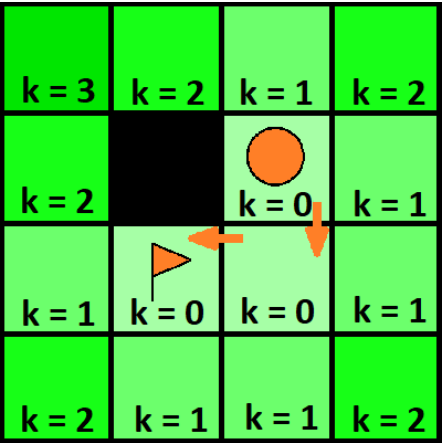
\includegraphics[scale=.4]{Images/RN-Explanation}}
\caption{The figure shows the number of deviating steps $k$ for each node. The node with $k=3$ would not be considered for the output because the robot only needs two steps to reach its goal. The image was taken from (CITE PAPER).}
\label{fig:rn}
\end{figure}

\section{Auxiliary Programs}
Apart from the ASP encoding, I have created several python programs which served different purposes during the project.
\subsection{Map Generator}
The map generator is used to create instances. The program can generate a map with a specified size in x- and y-direction. It also creates a specified amount of robots on random starting positions and the same amount of shelves that also have random starting positions. It can only create open maps which means that walls have to be edited in by hand. Specifying starting positions for robots or shelves is also impossible. The resulting file has a head in comment form which shows the chosen parameters, i.e. amount of nodes, robots, and so on. After that, all the nodes are initiated. Following that, each robot is initiated together with its shelf:
\begin{verbatim}
% Robot N
init(object(robot,N),value(at,(X1,Y1))).
init(object(shelf,N),value(at,(X2,Y2))).
\end{verbatim}
This way, controlling starting and goal position of a specific robot is easier when editing is required. The resulting file is called $instance.lp$.
\subsection{Solvers}
There are multiple solver programs. The simplest one is called $hor\_inc.py$. It can be used to solve a normal instance. It takes the solving ASP program and an input instance as input arguments. It then looks for the highest Manhattan distance between a robot and its goal position. This value is then taken as the constant $horizon$ for the ASP program. The program tries to solve the instance with this input. If the instance can be solved, it prints the solution and is finished. If the instance is considered unsatisfiable by clingo, it increases the $horizon$ by one and tries to solve it again. This is repeated until a solution is found or the horizon gets bigger than the number of nodes in the instance. The second case would mean that the instance is not solvable at all for an abstraction method because the robot could get to any position on the map it can reach. Another possibility for the program to end is if it takes longer than a specified time threshold. If it takes too long to solve and the threshold is reached, the python program stops the solving, and ``Timeout'' is printed. This solver was used to test the functionality of the abstraction methods. The other solvers were used for benchmarking the different methods. They are mostly the same as $hor\_inc.py$ with some extras. The exact usage will be discussed in the benchmarking section.
\subsection{Result Plotters}
There are two more python programs that I have created. Both are used to plot the benchmarking results. The first program, $lineg\_results.py$, takes the results for different methods for a specific instance, builds the average of these results, and plots a line graph for each method. To compare it to asprilo, the results for the asprilo benchmarking also need to be input as a method. The problem with this method is that the results can be strongly varying because there is a random element to the benchmarking. This is why the second program, $scatter\_results.py$, will be used to graphically show most of the results of the benchmarking. This program takes the different abstraction methods and directly compares them to the asprilo encoding. It creates a scatter plot which means that it is not necessary to calculate the average. This makes the analysis of the graphic much easier.  

\section{Benchmarking}
The idea for the benchmarking is to have maps of different sizes. On each map, the solver adds a robot, the ASP program tries to solve the instance and when it is done a new robot is added to the same map. This is done until a time limit is reached. The time limit chosen for this project is 10 minutes. This means that the benchmarking tests how many robots can be added in a time frame of 10 minutes. There are two different forms of adding robots. This is what the aforementioned python solvers are used for. The program $random\_benchmark\_solver.py$ uses an input instance that only has nodes and no robots or shelves at all. At the start and each time the solver finds a solution, the program randomly chooses a starting position for a robot and a shelf. This leads to a completely random instance. It is also possible to give the solver an argument that tells it which ``random seed'' it should use. In that case, the resulting instance is predetermined. The second benchmark solver is $preset\_benchmark\_solver.py$. This solver takes an instance where the robots and shelves are commented out at the start of the solving. It then incrementally adds these robots and shelves to the instance. This means that the instance is completely predetermined. The third solver is $combined\_solver.py$. This solver takes two programs and an instance as input. Since my programs only build an abstraction, they cannot be directly compared to a solving method. This is why this third solver first builds the abstraction and then uses the modified asprilo encoding, which was shown in a previous section, to solve this abstraction. The input instance looks the same as for the preset solver. This is done to ensure the satisfiability of the instance. This is necessary because the asprilo encoding is not made to use abstractions. That could lead to an abstraction being unsolvable. The following subsections will show the used map layouts and the results for each method. \\
The benchmarking was done on the HPC Turing of the university of Potsdam \cite{hpc}. A single run was calculated in sequential form. Each node of the cluster has 2 CPUs of the type Intel Xeon E5-2650v4, 64 GB of RAM, and an FDR Infiniband Adapter. All results can be found in the appendix.
\subsection{Map Layouts}
There are six map layouts used for the benchmarking. Each method was tested 10 times with preset starting coordinates and 10 times with random starting coordinates on each map. Some of the layouts were inspired by another paper \cite{mapf}. Three layouts are just an open map, which means that they have no inner walls. They have the sizes 16x16 nodes, 64x64 nodes, and 128x128 nodes. The preset coordinates for this type of map were chosen in a way that leads to at least one robot having the maximum amount of distance possible to its goal. The robots are added from left to right and top to bottom while the shelves are added the other way round. \\
The other map layout chosen is called ``rooms''. The sizes used for this type of map were 16x16 nodes, 32x32 nodes, and 64x64 rooms. The two bigger sizes were taken from the aforementioned paper. This includes the preset coordinates. The small size was created by myself. The starting coordinates of the robots and their goals were chosen in a way that had a preferably large discrepancy between the Manhattan distance and the number of steps needed to reach the goal. Images for all map layouts can be found in the appendix.
\subsection{Shortest Path}
This method was worse than the modified asprilo encoding in all instances. It could solve neither the preset instances of the medium- and large-sized open maps nor the preset instance of the large-sized rooms map. There were some random instances in those sizes that it could solve but the robot count was very low. The difference between the encoding for this method and the modified asprilo encoding mostly lies in the fact that this abstraction encoding does not have constraint rules for conflicts. The constraints likely help the solver to find the right plan faster. A look at the grounding times also seems to enforce this theory. In the medium-sized rooms map, this method could solve up to six robots. For the sixth robot, the solver needed about 175 seconds to find a solution. About 164 seconds of those were used to find a solution, while only 11 seconds were used for grounding. This shows that the grounding time is negligible compared to the solving time. Since the abstraction already takes longer than the complete solving, it was not necessary to test the abstraction together with the asprilo encoding. 
\subsection{Node Combining}
The Open Node Combining (ONC) method was only used for the open maps, while the Complete Node Combining (CNC) method was used for all maps. Using size 2x2 for combining in the ONC method shows that both methods have similar results on the open maps. Just looking at the abstraction time itself, both methods outperform the asprilo encoding by a large margin on small maps. Combining the abstraction with the solving shows that in the small-sized rooms map, CNC still yields better results than asprilo with a small number of robots. It makes sense that more robots mean a higher solving time increase for the combined solving instead of just using asprilo because a lot of robots mean only a small amount of nodes or no nodes at all get deleted. In bigger instances, using the combined solving is slower than asprilo. In the biggest instances, asprilo outperforms the abstraction time itself. However, using a bigger combining size for the ONC method shows that even in the largest open map, asprilo can be beaten. This means that the node combining method has a lot of potential and finding a way to optimize the combining size could be helpful. 
\subsection{Reachable Nodes}
The Reachable Nodes method has the worst results among the abstraction methods. It gets outperformed on every map. Similar to the Shortest Path method it cannot solve the preset instances of the maps with a size of 64x64 nodes and above. The times in the smaller maps are worse than the Shortest Path method. Taking a look at the grounding times in the medium-sized rooms map shows that the grounding times are at least as big as the solving time. The largest problem for this abstraction method is calculating the number of steps a node deviates from the shortest path. Since the method currently chooses the same node multiple times and looks for the minimum at the end, a lot of useless calculation is done. Finding a way around that should help with the solution time. Another way to improve the solution time could be finding a different upper limit for the number of deviating steps. Similar to the Shortest Path method, no combined solving was tested because the abstraction itself already took too long.

\section{Conclusion}
This paper showed my approach to finding a map abstraction for MAPF problems with ASP. I developed three different abstraction methods, with one method having two alternative versions. The Shortest Path and Reachable Nodes methods had worse solution times than the modified asprilo encoding, which means that these methods, at least in the form I used them, are not very useful for building abstractions. The Node Combining method shows much promise, especially if a way is found to optimize the size used for the combining. This means that map abstraction can have a positive influence on solving MAPF problems. However, it is likely only useful for instances where there are only a small amount of robots on a big map. If there are too many robots in an instance, the abstraction is not very useful because not many nodes can be ignored in that case. 
\newpage

\begin{thebibliography} {3}
\bibitem{my-git}
\begin{verbatim}
https://github.com/salewsky/MAPF-Project
\end{verbatim}

\bibitem{tarek-git}
\begin{verbatim}
https://github.com/tramadan-up/mapf-ba
\end{verbatim}

\bibitem{asprilo}
\begin{verbatim}
https://potassco.org/asprilo/
\end{verbatim}

\bibitem{mapf}
Stern et al. (2019). Multi-Agent Pathfinding: Definitions, Variants, and Benchmarks. Symposium on Combinatorial Search (SoCS), 151-158.

\bibitem{asp}
Janhunen, T., and Niemelä, I. (2016). The Answer Set Programming Paradigm. AI Magazine, 13-24.

\bibitem{clingo}
Gebser et al. (2010). A User's Guide to gringo, clasp, clingo, and iclingo. 

\bibitem{nc1}
Sturtevant, N., and Buro, M. (2005). Partial Pathfinding Using Map Abstraction and Refinement. Proceedings of AAAI, 47-52.

\bibitem{nc2}
Sturtevant, N. and Buro, M. (2021). Improving Collaborative Pathfinding Using Map Abstraction. Proceedings of the AAAI Conference on Artificial Intelligence and Interactive Digital Entertainment, 2(1), 80-85.

\bibitem{rn}
Husár et al. (2022). Reduction-based Solving of Multi-agent Pathfinding on Large Maps Using Graph Pruning. AAMAS 2022.

\bibitem{hpc}
\begin{verbatim}
https://www.cs.uni-potsdam.de/bs/research/labs.html#turing
\end{verbatim}

\end{thebibliography}

\newpage
\appendix

\section{Map Layouts}

\subsection{Open Maps}
Since the only difference between the maps is the size, only images for the small open map is shown.
\begin{figure}[H]
\centering{
\includegraphics[scale=.4]{Images/Small-Open}}
\caption{The map layout for the open 16x16 map}
\end{figure}
\begin{figure}[H]
\begin{minipage}{.4\linewidth} 
\centering{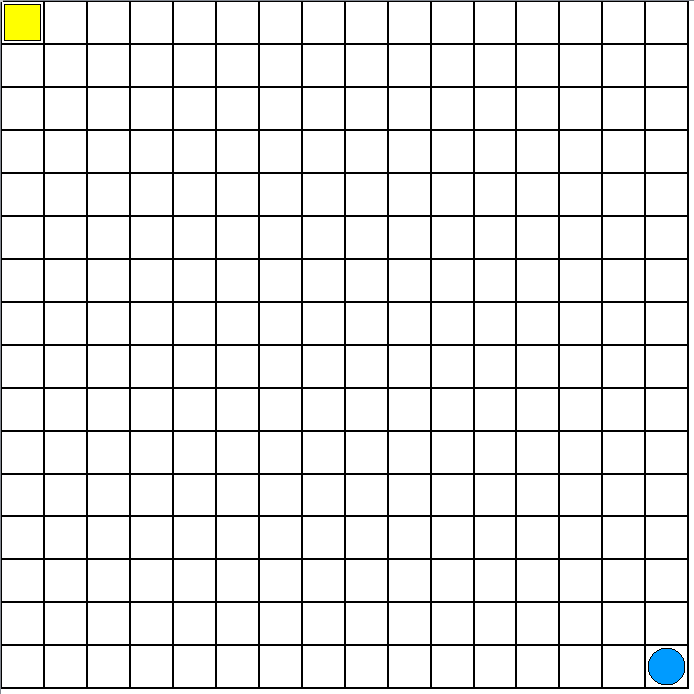
\includegraphics[scale=.2]{Images/Small-Open-1R}}
\caption{The small open map with 1 robot activated}
\end{minipage}
\hspace{2cm}
\begin{minipage}{.4\linewidth} 
\centering{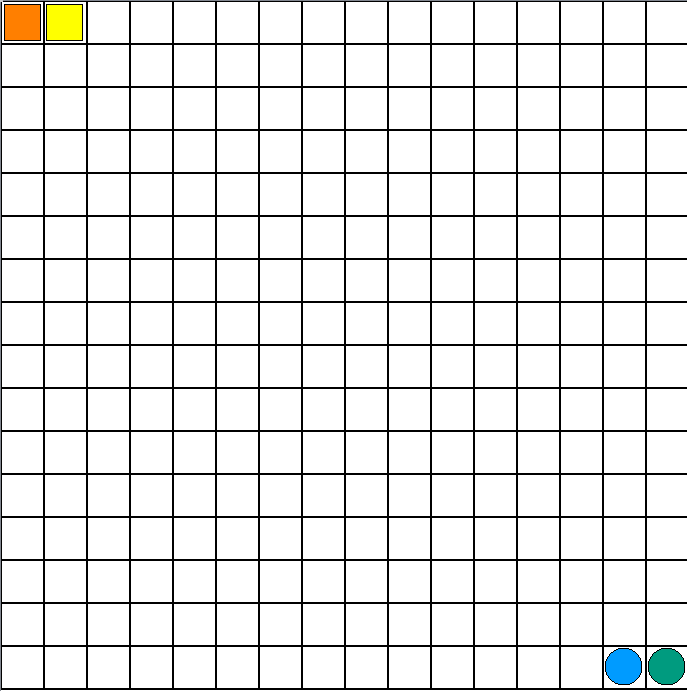
\includegraphics[scale=.2]{Images/Small-Open-2R}}
\caption{The small open map with 2 robots activated}
\end{minipage}
\end{figure} 

\subsection{Room Maps}
\begin{figure}[H]
\centering{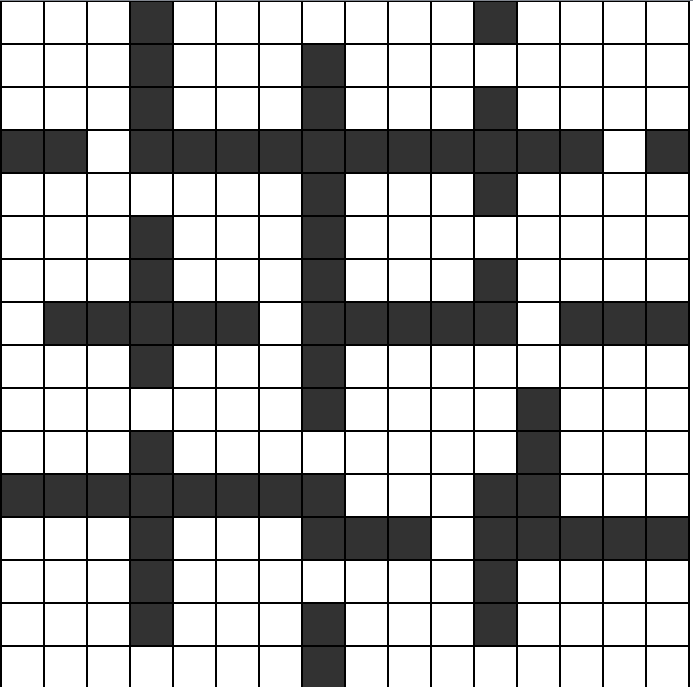
\includegraphics[scale=.4]{Images/Small-Rooms}}
\caption{The map layout for the 16x16 rooms map}
\end{figure}
\begin{figure}[H]
\centering{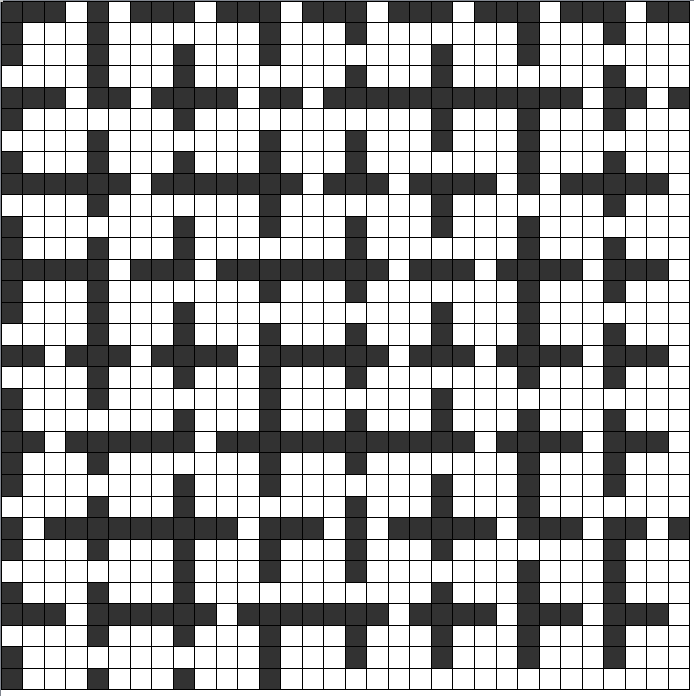
\includegraphics[scale=.4]{Images/Medium-Rooms}}
\caption{The map layout for the 32x32 rooms map}
\end{figure}
\begin{figure}[H]
\centering{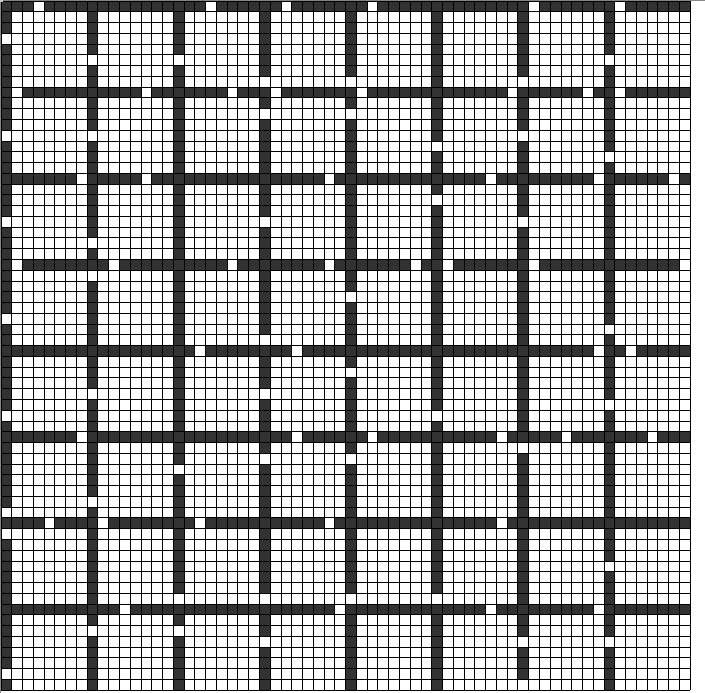
\includegraphics[scale=.4]{Images/Large-Rooms}}
\caption{The map layout for the 64x64 rooms map}
\end{figure}

\newpage

\section{Benchmark Results}
\subsection{Small Rooms}
\begin{figure}[H]
\centering{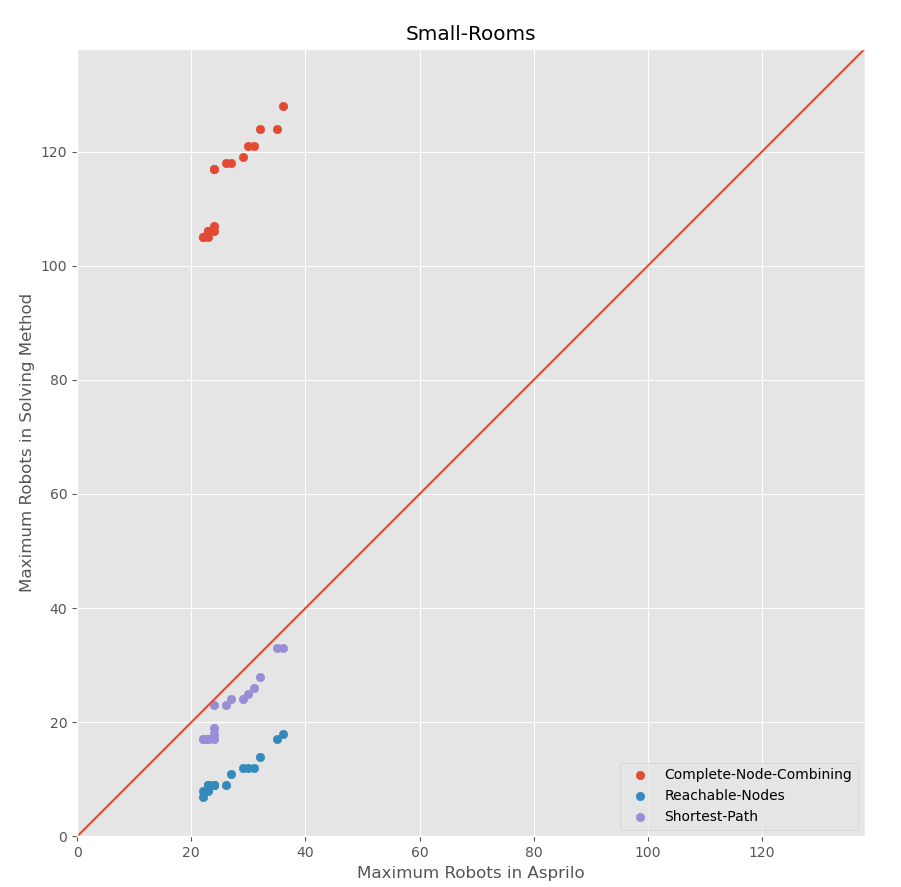
\includegraphics[scale=0.35]{Images/Results-Small-Rooms-1}}
\caption{Results for Complete Node Combining, Shortest Path, and Reachable Nodes}
\end{figure}
\begin{figure}[H]
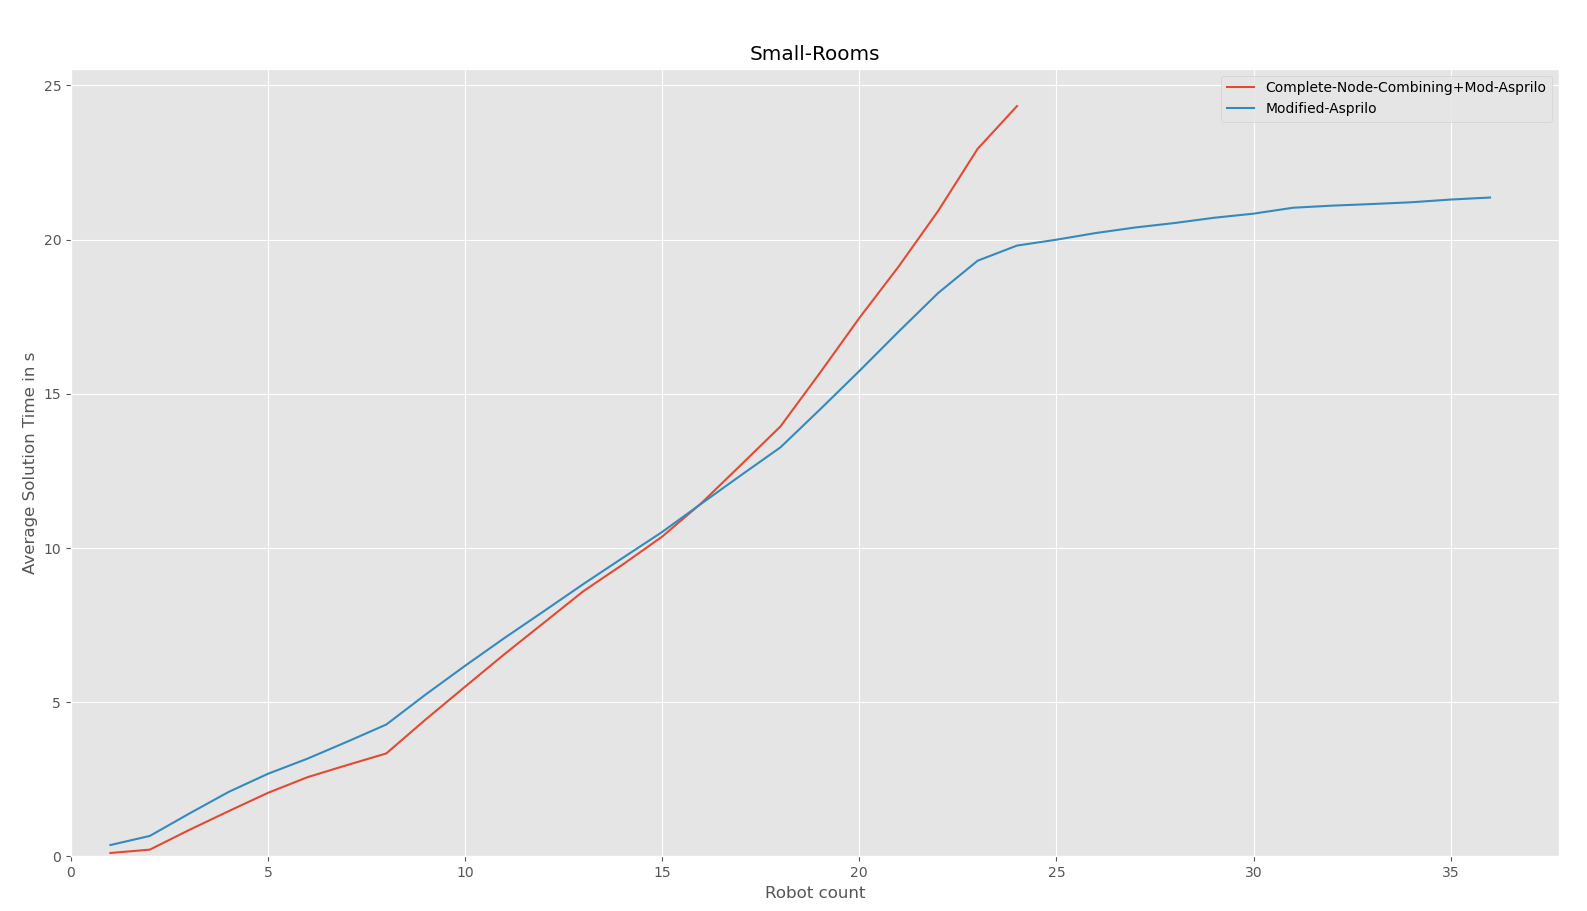
\includegraphics[scale=0.35]{Images/Results-Small-Rooms-2}
\caption{Results for Complete Node Combining together with asprilo}
\end{figure}

\subsection{Small Open}
\begin{figure}[H]
\begin{minipage}{.4\linewidth} 
\centering{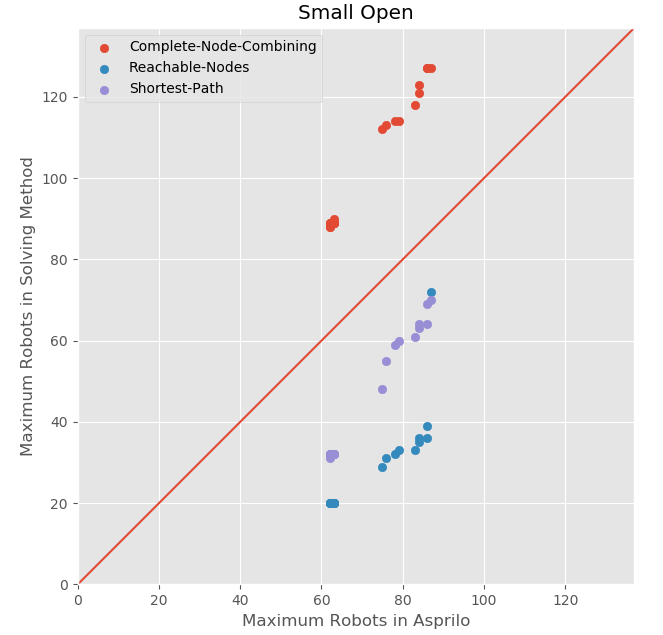
\includegraphics[scale=.4]{Images/Results-Small-Open-1}}
\caption{Results for Complete Node Combining, Shortest Path, and Reachable Nodes}
\end{minipage}
\hspace{1.5cm}
\begin{minipage}{.4\linewidth} 
\centering{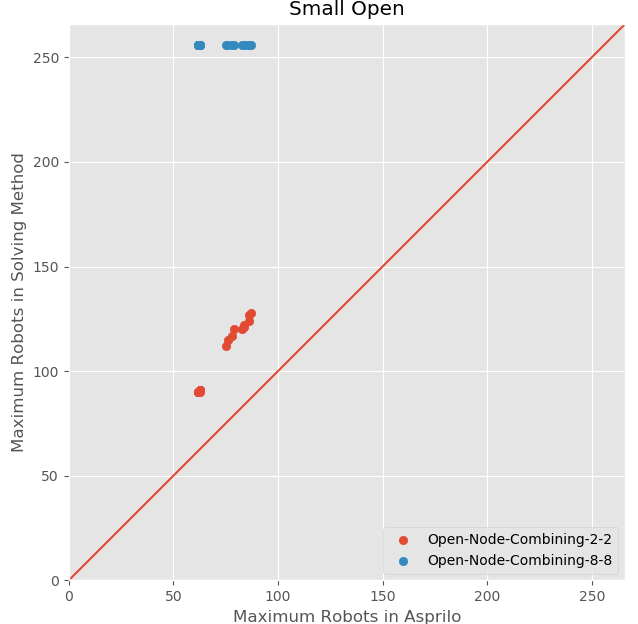
\includegraphics[scale=.4]{Images/Results-Small-Open-2}}
\caption{Results for Open Node Combining sizes 2x2 and 8x8}
\end{minipage}
\end{figure} 
\begin{figure}[H]
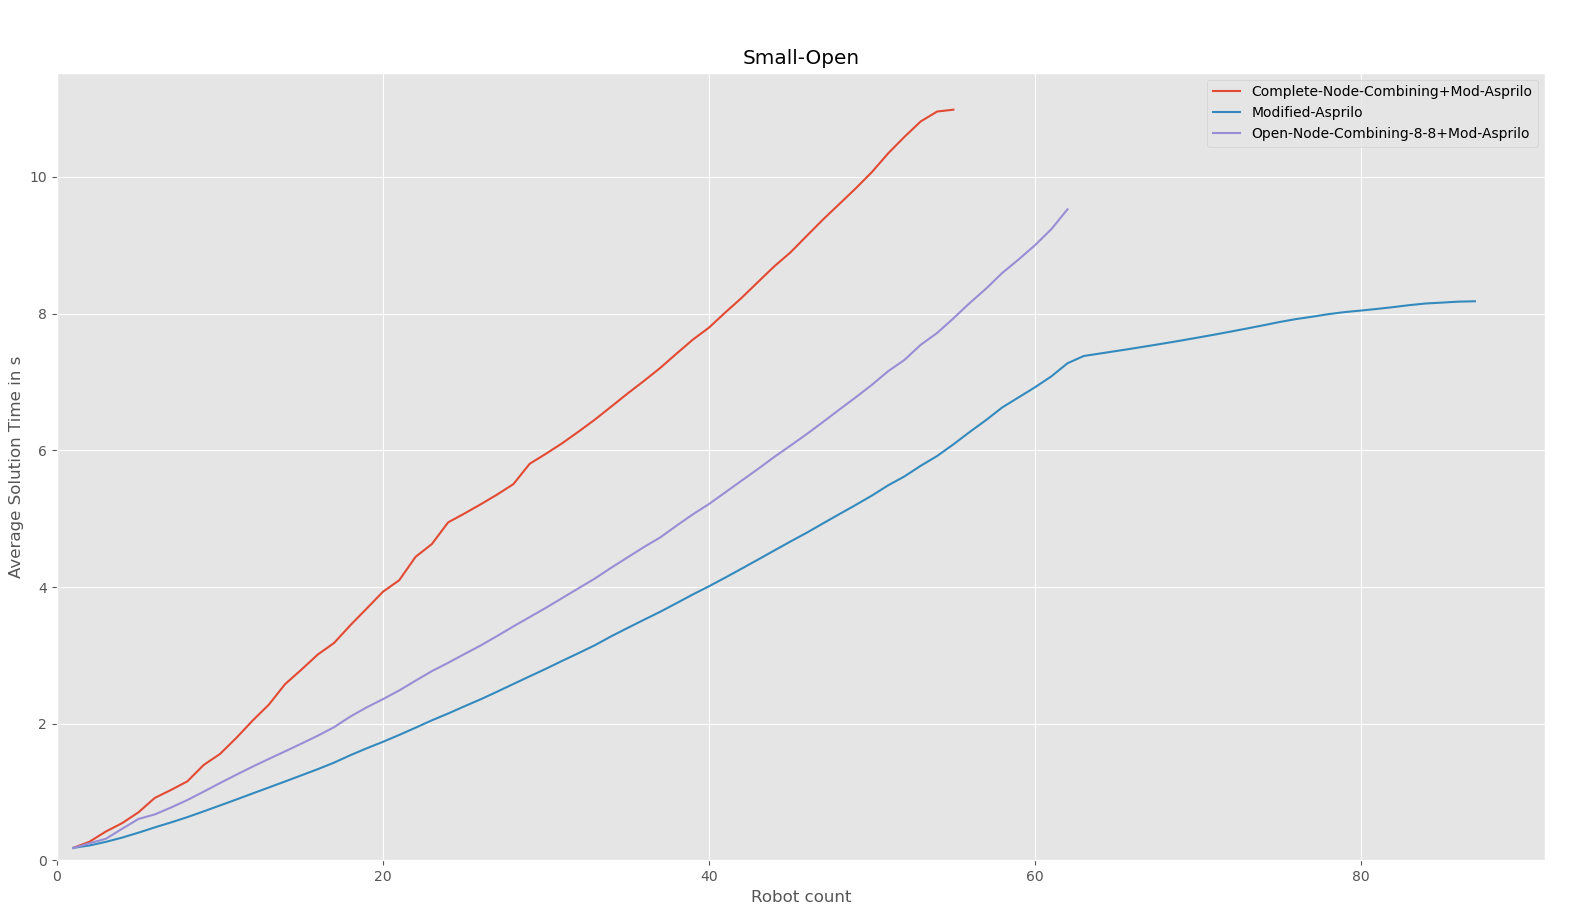
\includegraphics[scale=0.4]{Images/Results-Small-Open-3}
\caption{Results for Complete Node Combining and Open Node Combining together with asprilo}
\end{figure}

\subsection{Medium Rooms}
\begin{figure}[H]
\centering{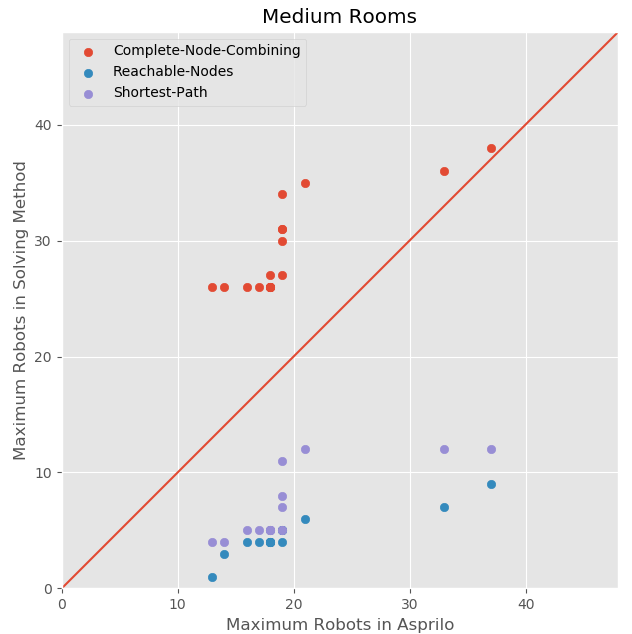
\includegraphics[scale=0.4]{Images/Results-Medium-Rooms-1}}
\caption{Results for Complete Node Combining, Shortest Path, and Reachable Nodes}
\end{figure}
\begin{figure}[H]
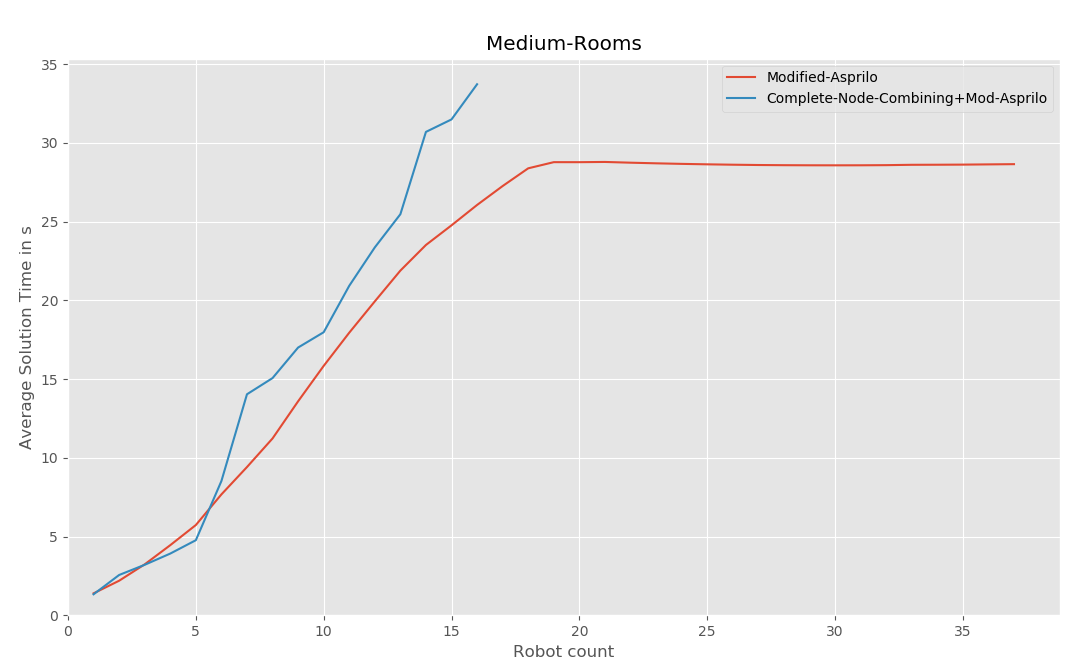
\includegraphics[scale=0.4]{Images/Results-Medium-Rooms-2}
\caption{Results for Complete Node Combining together with asprilo}
\end{figure}


\subsection{Medium Open}
\begin{figure}[H]
\begin{minipage}{.4\linewidth} 
\centering{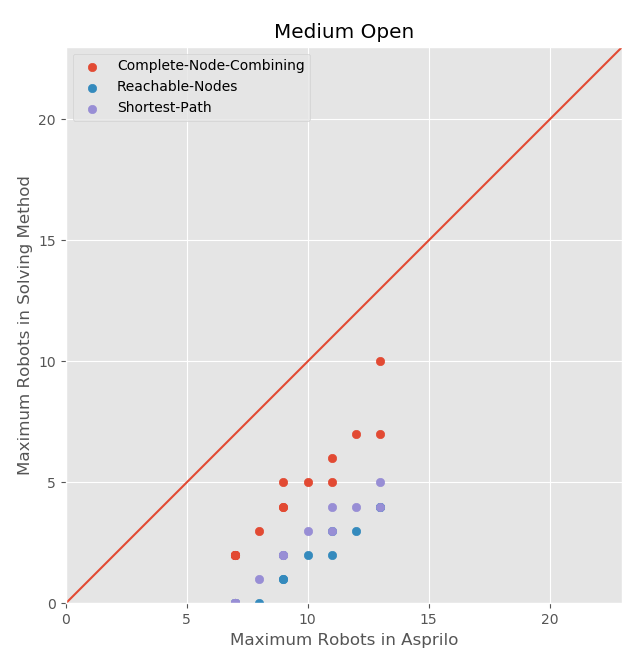
\includegraphics[scale=.4]{Images/Results-Medium-Open-1}}
\caption{Results for Complete Node Combining, Shortest Path, and Reachable Nodes}
\end{minipage}
\hspace{1.5cm}
\begin{minipage}{.4\linewidth} 
\centering{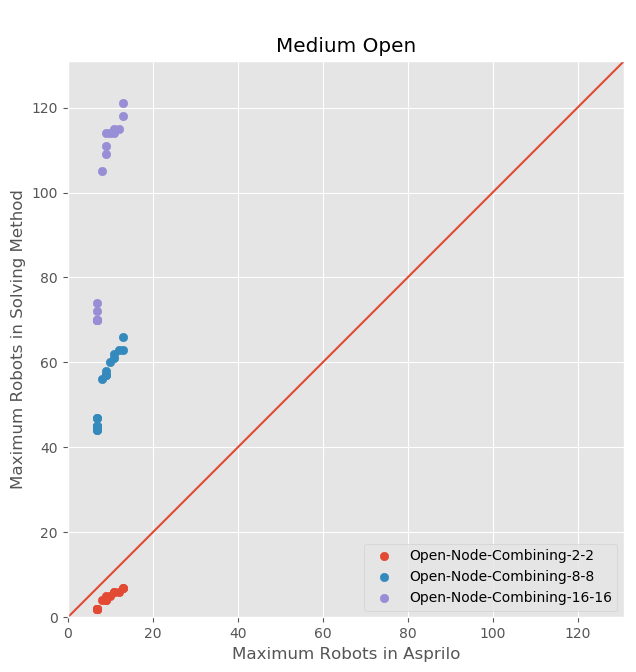
\includegraphics[scale=.4]{Images/Results-Medium-Open-2}}
\caption{Results for Open Node Combining sizes 2x2, 8x8, and 16x16}
\end{minipage}
\end{figure} 
\begin{figure}[H]
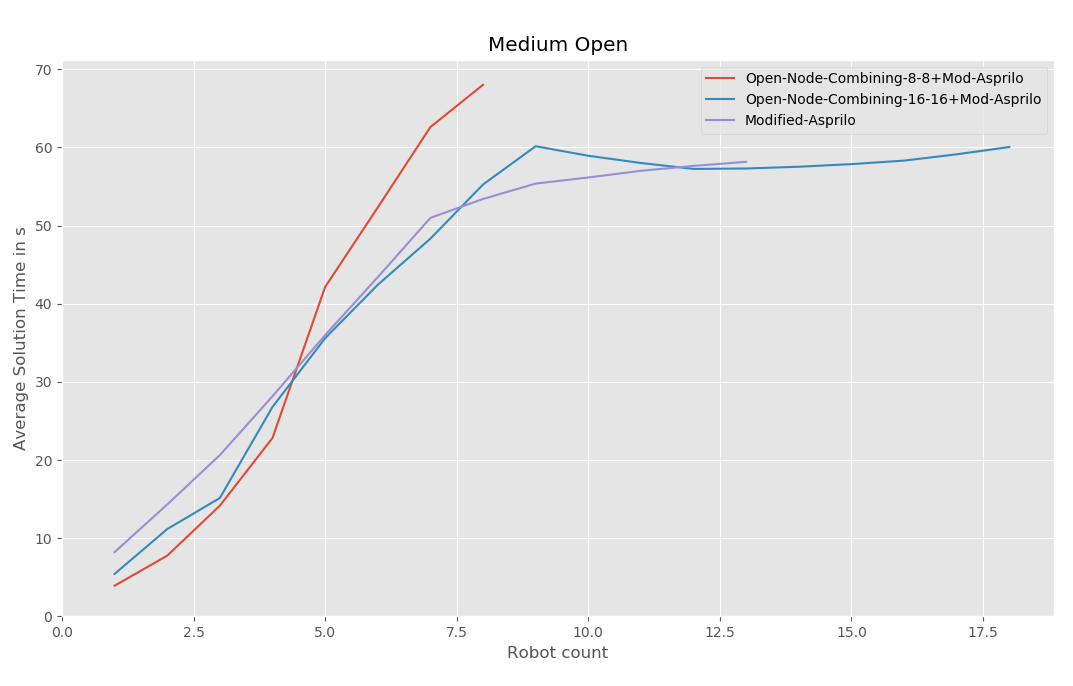
\includegraphics[scale=0.4]{Images/Results-Medium-Open-3}
\caption{Results for Open Node Combining together with asprilo}
\end{figure}

\subsection{Large Rooms}
\begin{figure}[H]
\centering{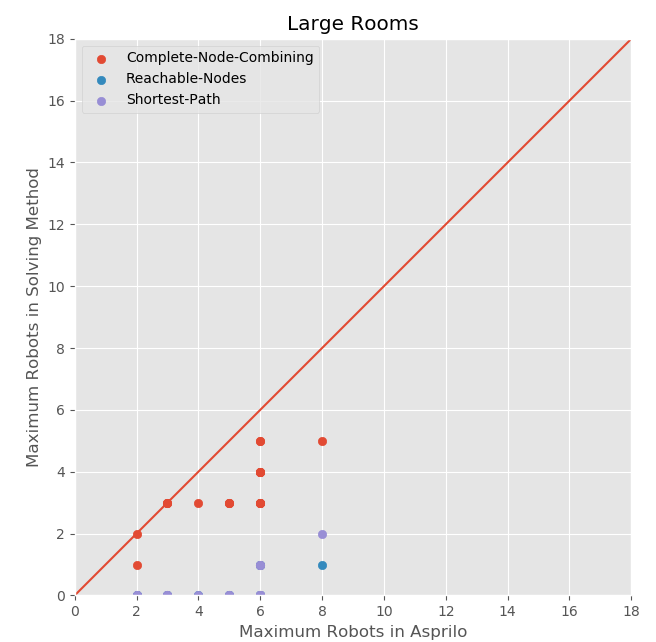
\includegraphics[scale=0.4]{Images/Results-Large-Rooms-1}}
\caption{Results for Complete Node Combining, Shortest Path, and Reachable Nodes}
\end{figure}

\subsection{Large Open}
\begin{figure}[H]
\begin{minipage}{.4\linewidth} 
\centering{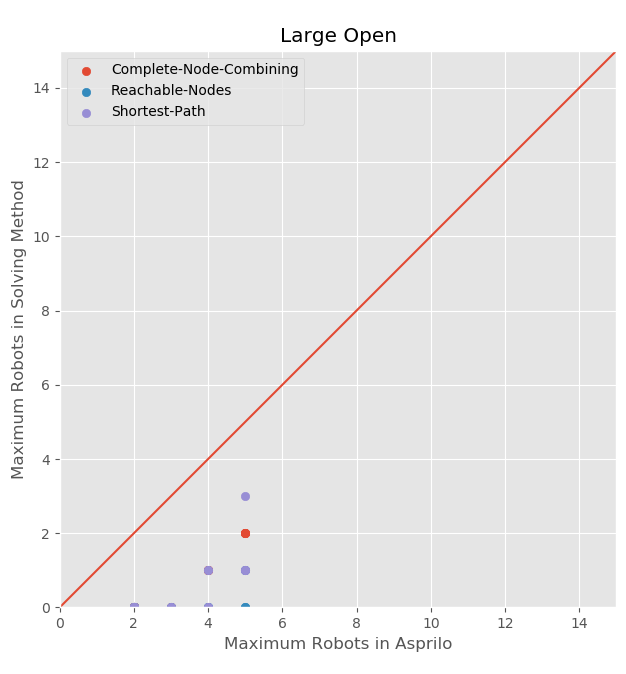
\includegraphics[scale=.4]{Images/Results-Large-Open-1}}
\caption{Results for Complete Node Combining, Shortest Path, and Reachable Nodes}
\end{minipage}
\hspace{1.5cm}
\begin{minipage}{.4\linewidth} 
\centering{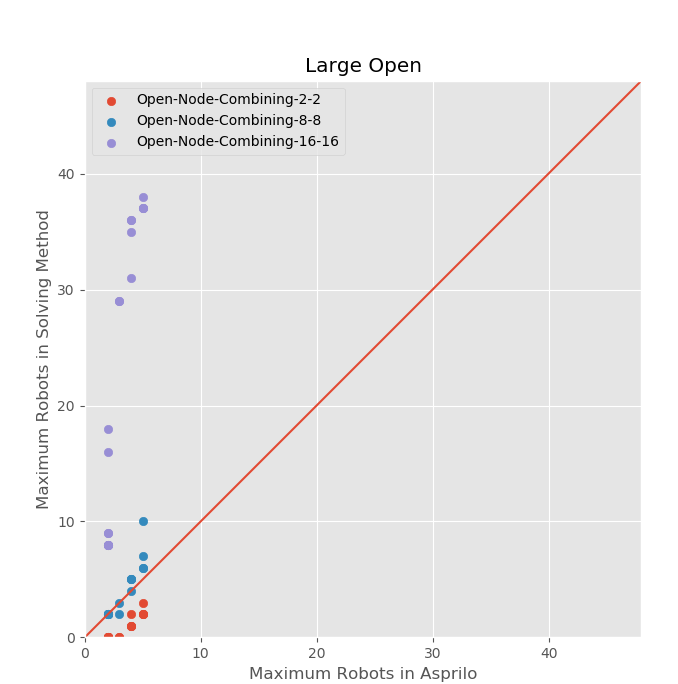
\includegraphics[scale=.4]{Images/Results-Large-Open-2}}
\caption{Results for Open Node Combining sizes 2x2, 8x8, and 16x16}
\end{minipage}
\end{figure} 
\begin{figure}[H]
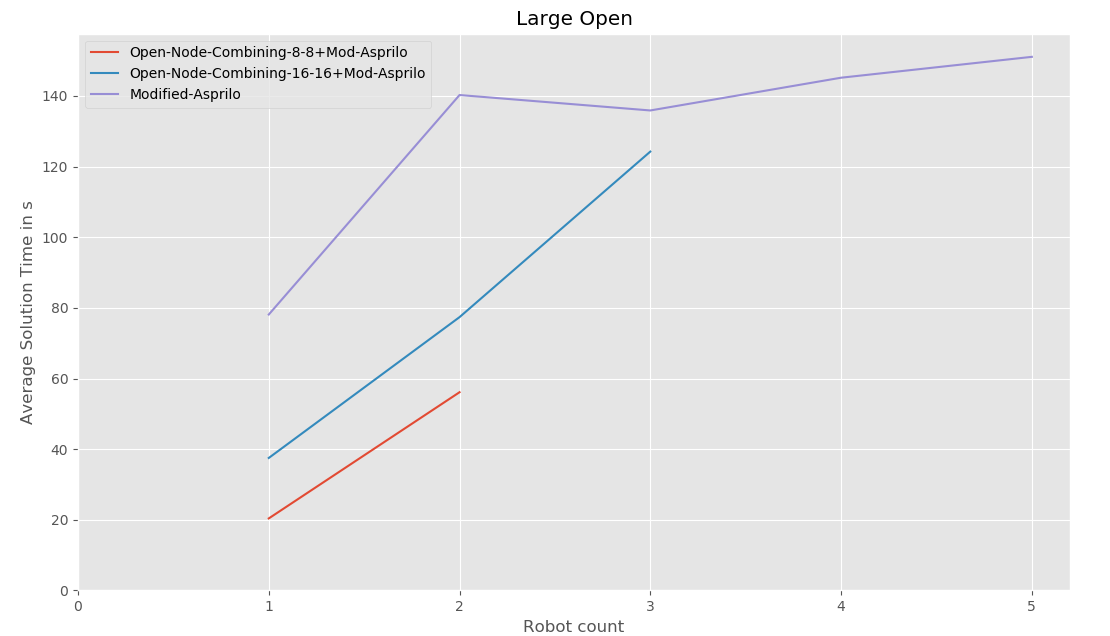
\includegraphics[scale=0.4]{Images/Results-Large-Open-3}
\caption{Results for Open Node Combining together with asprilo}
\end{figure}
\newpage
\section{Affidavit}
I hereby affirm that this Bachelor's Thesis represents my written work and that I have used no source and aids other than those indicated.
All passages quoted from publications or paraphrased from these sources are properly cited and attributed.
\vspace{\baselineskip}
\vspace{\baselineskip}
\vspace{\baselineskip}
\vspace{\baselineskip}

\noindent\begin{tabular}{lll}
\makebox[5cm]{\hrulefill} & \hspace{2cm} & \makebox[5cm]{\hrulefill}\\
Date, Place &  & Signature 
\end{tabular}

\end{document}